\documentclass{article}
\author{Richard Gendal Brown, James Carlyle, Ian Grigg, Mike Hearn}
\date{May, 2018}
\title{The Corda Platform: An Introduction}
\usepackage{amsfonts}
\usepackage{listings}
\usepackage{color}
\usepackage{epigraph}
\usepackage{graphicx}
\graphicspath{ {images/} }
\usepackage[export]{adjustbox}
\usepackage{float}
\usepackage{hyperref}
\usepackage[super,comma,sort&compress]{natbib}
\usepackage[nottoc]{tocbibind}
\renewcommand{\thefootnote}{\alph{footnote}}
\setlength\epigraphwidth{4.5cm}
\setlength\epigraphrule{0pt}
% Get rid of ugly boxes around clickable links
\usepackage{xcolor}
\hypersetup{
colorlinks,
linkcolor={blue!50!black},
citecolor={blue!50!black},
urlcolor={blue!80!black}
}

\begin{document}

\maketitle 

\begin{abstract}

A distributed ledger made up of mutually distrusting nodes would allow for a single global database that records the state of deals, obligations and other agreements between institutions and people. This would eliminate much of the manual, time consuming effort currently required to keep disparate ledgers synchronised with each other. It would also allow for greater levels of code sharing than is currently typical in the financial and other industries, reducing transactions costs for everyone. We present Corda, a software implementation which is designed to achieve these goals, and a network to which Corda nodes deployed by a broad range of operators can be connected to be assured of mutual interoperability. This paper provides a high level introduction intended for the general reader and supersedes its predecessor, `Corda: An Introduction'\cite{CordaIntro}. A companion technical white paper\cite{CordaTech} elaborates on the design and fundamental architectural decisions.
\end{abstract}
\newpage
\tableofcontents
\newpage
\section{Introduction}
We envision a future where legal agreements such as business contracts are recorded and automatically managed without error, where anybody can transact seamlessly for any contractual purpose without friction. We believe markets will move towards models where parties to contracts collaborate to maintain accurate, shared records rather than maintaining their own independent and inconsistent systems which require extensive reconciliation processes to ensure consistency. Duplicates, reconciliations, failed matches and breaks will be things of the past. Isolated pools of trapped assets will be no more.

This paper introduces the Corda platform. The Corda platform consists of an open source software project, Corda, and a set of standards, network parameters and associated governance processes, which together define the global Corda Network. Collectively, they enable any organisation or individual on this open network to transact directly with any other. Uniquely, this architecture is designed to model and automate real-world transactions in a legally enforceable manner, and do so across an open network on which multiple applications can execute and seamlessly interoperate. It does so whilst placing identity, transaction finality, privacy and open governance at its core.

The end state vision is one where real-world entities manage legally-enforceable contracts, and transfer value without technological constraints or loss of privacy. In contrast to `unpermissioned' blockchain platforms, the Corda platform is intended to manage real-world transactions between identifiable parties, with privacy and legal certainty. In contrast to other `permissioned' blockchain platforms, the Corda Platform is intended to allow multiple groups of participants (and associated applications) to co-exist and interoperate across the same open network. The network's governance model is explicitly designed to reflect the common interests of the diverse user-base of the platform.

To facilitate settlement of obligations arising from contracts managed on the platform, the Corda platform enables the issuance, transfer and redemption of cash-like liabilities denominated in real-world currencies where regulation allows. In addition, the architecture enables the issuance of native assets and tokens on the platform which can be used to incentivise adoption and participation, pay for services and can be either platform-wide or specific to particular Business Networks\footnote{See section \ref{businessnetworks} for a definition} operating on the broader Corda network.

This paper introduces the design features of the Corda platform which we believe make it an attractive choice for anybody seeking to record, manage and automate real-world agreements across the internet without friction.\footnote{The author can be reached via email: Richard Gendal Brown \href{mailto:richard@r3.com}{(richard@r3.com)}. This paper builds on its predecessor, which was  authored by Richard Brown, James Carlyle, Ian Grigg and Mike Hearn. In addition, the author is grateful to Nick Arini, Dave Hudson, Nigel King, Todd McDonald and Mike Ward for input to and review of this paper.}.

\section{Context}
Corda has been open source software since 2016. The design of Corda has benefitted from the collaboration of a global and diverse alliance of organisations representing many industries, and regulatory engagement has been a key element of this design process\footnote{Many of the individuals and firms who contributed to the design and development of Corda are listed at \url{https://github.com/corda/corda/blob/master/CONTRIBUTORS.md}.}. The requirements of the financial industry formed the original basis of Corda's design but field experience has demonstrated that Corda has broad applicability, well beyond banking.

The motivating problem, which Corda seeks to solve, is the problem of managing contracts and other agreements between any combination of firms and individuals, especially when those parties trust each other enough to trade but not enough to have their counterparty maintain all the records.

Regardless of industry or geography, we see the same inefficient pattern in today's business environment: institutions invariably maintain their own ledgers, which record each firm's view of its agreements and positions with respect to its customer set and its trading partners. This duplication can lead to inconsistencies, and it drives a need for costly matching, reconciliation and fixing of errors by and among the various parties to a transaction. To the extent that differences remain between two firms' views of the same transaction, this is also a source of risk, some of it potentially systemic.

Until recently, this was unavoidable: except for centralised market infrastructures\footnote{Examples of this in the financial industry include the Depository Trust \& Clearing Corporation (DTCC) and Continuous Linked Settlement Group (CLS), and there are equivalents in many other industries}, there were few effective ways to consolidate technology across firms without also consolidating the firms themselves.

Centralised market infrastructure utilities have gone some way towards increasing the amount of data and business-logic sharing between firms. But this development creates unfavourable tradeoffs of its own: such as the possibility of rent-seeking and inertia. This has been evidenced by how the world of financial transactions still lags far behind that which has been achieved in the realm of consumer and web based software since the advent of the web.

We believe that the maturation of cryptographic techniques, exemplified in part by what is commonly referred to as ``blockchain technology", provides a new opportunity. This is the possibility of authoritative systems of record that are securely shared between firms, and which enable a large subset of each firm's transactions to be managed in a common way. Systems that provide a guarantee that ``I know that what I see is what you see".

This vision is in contrast to today, where a multitude of expensive, non-interoperable, isolated systems drive up cost, risk, duplication and error. In essence, we foresee a transition from IT infrastructures that are developed and optimised at the level of individual firms to IT infrastructures that are developed and optimised at the level of markets and industries.

\section{Vision}
In the long-term, one can envision a shared ``global logical ledger" with which all economic actors (companies, individuals, machines) will interact and which will allow any parties to record and manage agreements amongst themselves in a secure, consistent, reliable, private, auditable and authoritative manner.

A possible end-state is one in which we have moved from authoritative systems-of-record maintained \textit{within} firms, and which must then be expensively reconciled, to global authoritative systems-of-record shared \textit{between} all economic actors: optimisation at the level of markets, not at the level of firms.

This vision provides the opportunity to transform the economics of firms by implementing a new shared platform for the recording of commercial agreements and processing of business logic: one where a single global logical ledger is authoritative for all agreements between participants recorded on it. This architecture defines a new shared platform for all industries, upon which incumbents, new entrants and third parties can compete to deliver innovative new products and services.

Importantly, the vision is one in which a large number of firms, suppliers, customers and third parties manage a large and diverse range of agreements on the \textit{same} platform, through deployment of a large range of Corda Applications, or \textit{CorDapps}, across a common, shared, openly governed network. Corda is designed to allow information and assets gained through usage of one CorDapp to be used in a different context with different counterparties in a different CorDapp. This stands in contrast with other enterprise-focussed blockchain platforms, which are designed to be deployed as isolated instances for each supported application.

\begin{figure}[H]
    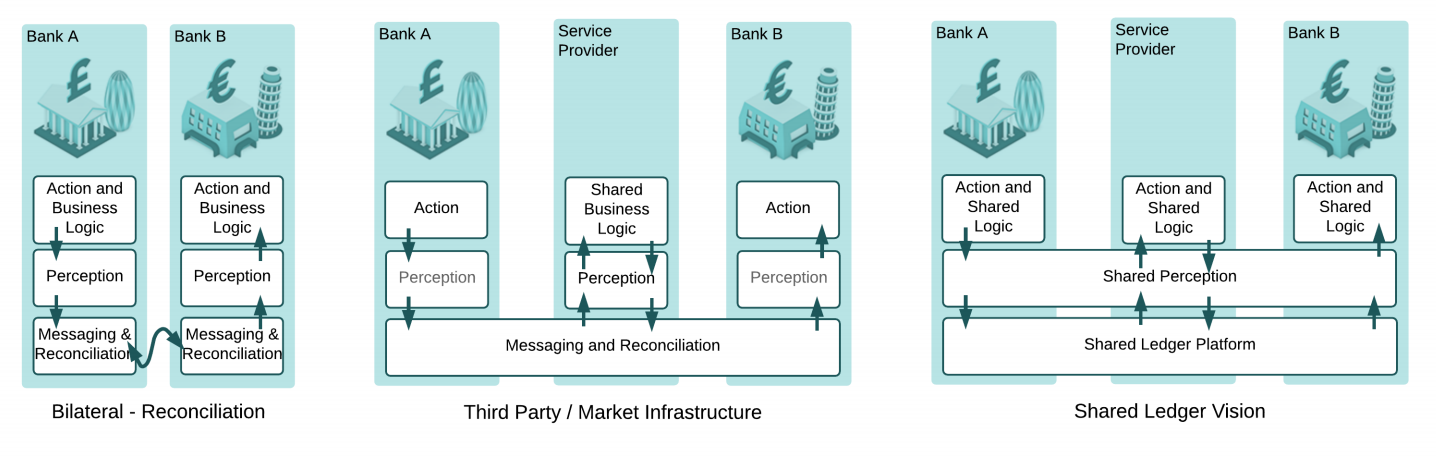
\includegraphics[scale=.5, center]{sharedlogic}
    \caption{In the diagram above, we show a progression from a world where parties to shared facts record and manage their own records, with associated discrepancies and duplications (\textit{``Bilateral - Reconciliation"}) or one where parties delegate control and responsibility over critical processing to centralised utilities (\textit{``Third Party / Market Infrastructure"}), to one where they collaborate to maintain a shared record, assured to be consistent between them, consuming the services of existing and new service providers and market infrastructure providers on an open and competitive basis (\textit{``Shared Ledger Vision"}).}
\end{figure}

We believe that the savings accruing from higher-quality data, fewer discrepancies and quicker agreement of details between firms will be significant. Moreover, deployment of this common architecture across firms will define a new platform on which existing and new providers can compete to serve the needs of clients. Going further, it is possible that such a platform will also find application within firms, where the problem of multiple systems recording details of the same trades is also a major driver of cost and complexity.

However, it is also important to ensure that the mistakes associated with new technology introduction in the past are not repeated. Isolated, non-interoperable, standalone deployments help nobody. The Corda vision is one where \textit{multiple} applications, products and services are deployed to an openly governed \textit{common shared network}, where assets gained in one context from one trading partner for one service can be immediately redeployed without friction or transfer costs for another purpose to pay a different trading partner utilising a different application. To achieve this, different solutions utilising Corda software need to share some common standards and agree on some common parameters. This common layer of standards, underpinned by open, transparent governance over their evolution, defines the global Corda \textit{network}.

\subsection{End-State Principles}
Business principles underpinning our end-state vision using the Corda platform include:
\begin{itemize}
    \item Inclusion. Parties are able to discover each other freely, and transact directly, in a single, open network.
    \item Assured identity. Parties will have assurance over the identity of participants in the network.
    \item Privacy. The only parties who have access to the details of a transaction are those who participate in the transaction and those who need to assure themselves of transaction provenance.
    \item Shared logic. The behavior of agreements managed by the system will be described in computer code that is shared to ensure consistency and validity of agreements.
    \item Legal footing. Deals recorded by the ledger are, by contract, accepted as admissible evidence and legally binding by all parties in any dispute.\cite{Ricardian}
	\item Authoritative. Facts recorded by the ledger are regarded as authoritative rather than ``shadows" of authoritative data held elsewhere.
	\item Immutability. Facts recorded on the ledger are final and immutable; errors and unwinds must be processed through a subsequent transaction.
    \item Open. The system is open: open source, participation, development, governance and standards to ensure the platform balances the needs of its diverse user-base in a transparent fashion.
\end{itemize}
\paragraph{}

Architectural choices underpinning the vision include:
\begin{itemize}
    \item Scale. The network will scale to support billions of transactions daily across industries.
    \item Longevity. Different versions of Corda will be able to coexist on the same network and applications will continue to run on later versions.
    \item Secure. This system will operate under the assumption of an adversarial security environment.
    \item Stable. The network will evolve carefully, with consensus-critical \textit{``network parameters"} maintained through a transparently governed process.
    \item Interoperable. The platform is designed to allow multiple applications to coexist and interoperate on the same network; a standardised set of interfaces for contracts are included to maximise interoperability from a diverse range of providers; the Corda software is implemented on industry-standard tools to maximise deployability and integration with existing enterprise infrastructures.
\end{itemize}

We will measure successful delivery of this vision through the reduction of cost, risk and regulatory burden, through the introduction of innovative new products and services by third parties, and by the diversity and scale of the ecosystem this enables.

From our requirements analysis and assessment of existing distributed ledger platforms, we concluded that no existing platform could deliver these end-state principles. For example, the threat models underpinning the designs of traditional distributed databases were unsuitable for our use-case of bringing mutually distrusting legal entities into consensus across the internet; such systems assume a common, fully trusted, administrative domain. The architectures of existing blockchain systems such as Ethereum were unsuitable for our requirement of restricted and carefully specified data sharing at the level of individual legal agreements with legal enforceability.

As a result we present the Corda platform.

\section{Corda}
Corda is distributed ledger software for recording and processing shared data such as contracts, designed to implement the vision contained in this document.

Corda supports smart contracts, matching the definition of Clack, Bakshi, Braine\cite{SCT}; our smart contract is an agreement whose execution is both \textit{automatable} by computer code working with human input and control, and whose rights and obligations, as expressed in legal prose, are legally \textit{enforceable}.

\subsection{Principal Features}
Corda's design was initially driven by the needs of regulated financial institutions but turns out to be far more broadly applicable. It is heavily inspired by blockchain systems, but without the design choices that make traditional blockchains inappropriate for the execution of real-world business transactions.

Our fundamental building block is a \textit{``state object"}, representing a specific instance of a specific agreement, which may be thought of as representing a real-world contract or section of a contract. We use the terms `agreement' and `contract' interchangeably in this paper. This stands in contrast to systems where the data over which participants must reach consensus is the state of an entire ledger or the state of an entire virtual machine. Corda provides three main tools to achieve global distributed consensus:
\begin{itemize}
    \item \textit{Smart contract} logic which specifies \textit{constraints} that ensure state transitions are valid according to pre-agreed \textit{rules}, described in \textit{contract code} as part of \textit{CorDapps}.
    \item Uniqueness and timestamping services known as \textit{notary pools} to order transactions temporally and eliminate conflicts.
    \item A unique component called the \textit{flow framework} which simplifies the process of writing complex multi-step protocols between multiple mutually distrusting parties across the internet.
\end{itemize}

\subsection{Concepts}
We begin with the idea of a global ledger: a reliable single source. However, in our model, it is not the case that transactions and ledger entries are globally visible. A transaction between a group of parties is visible only to them, and to those whose own view of the ledger in the future may depend on verifying the validity of this transaction. This contrasts with platforms based on global broadcast but also with platforms with an approach to privacy that depends on partitioning data into coarse-grained ``confidential contracts" or ``channels". Such designs logically cannot support a global network that supports multiple interoperable applications and assets.

The foundational object in our concept is a \textit{state object}, which is a digital document which records the existence, content and current state of an agreement between two or more parties. It is intended to be shared only with those who have a legitimate reason to see it. To ensure consistency in a global, shared system where not all data is visible to all participants, we rely heavily on secure cryptographic hashes to identify parties and data, and to link states to previous versions to provide chains of provenance. The ledger is defined as a set of immutable state objects.

We talk and think in terms of the `state' of `agreements'. That is: not just a contract between parties but a specific instance, version and current status of that contract. Our objective is to ensure that all parties to an agreement remain in consensus on these facts as they evolve and is intended to interface naturally with real-world legal systems where required. We believe this is the essence of the blockchain concept that is fundamental to its adoption by real-world businesses. Corda ensures that the data held by different actors is, and remains, consistent as operations are applied to update that data. This forms a foundation on which reliable transactions can be built: from simple monetary payments to sophisticated smart contracts.

\begin{figure}[H]
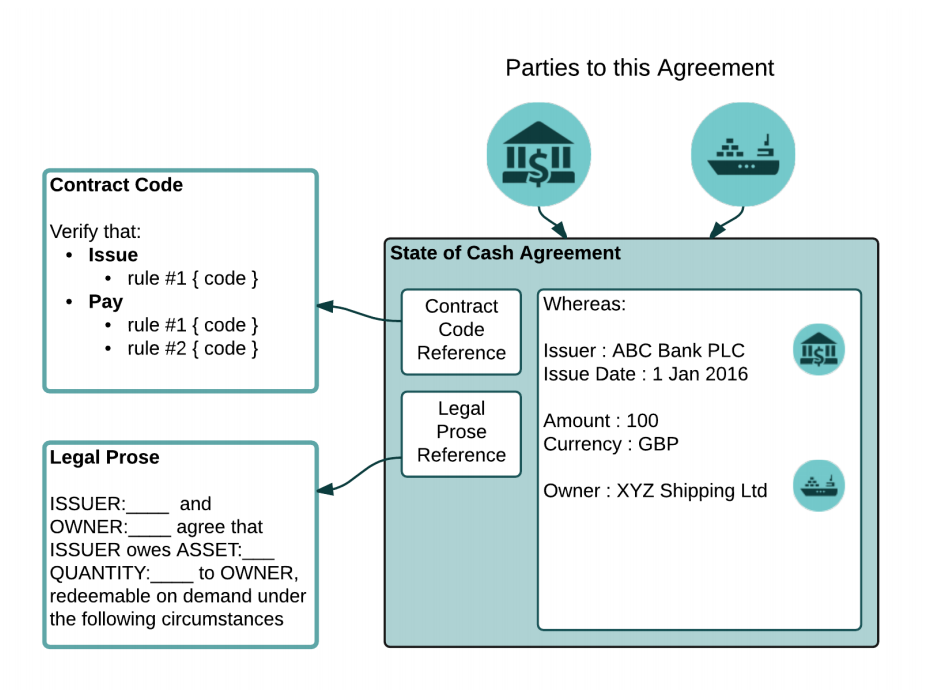
\includegraphics[scale = .4, center]{partiesto}
\caption{In the diagram above, we see a state object representing a deposit of \pounds100 at a commercial bank, owned by a fictional shipping company. The state object refers to the contract code that governs its transitions, which is likely to be written once and reused by huge numbers of states, and can refer by hash to its governing legal prose.}
\end{figure}

\subsection{Consensus}
In Corda, updates are applied using \textit{transactions}, which consume existing state objects and produce new state objects, thus creating chains of provenance. There are two aspects of consensus:
\begin{enumerate}
\item{Transaction validity: parties can reach certainty that a proposed update transaction defining output states is valid by checking that the associated contract code, which is required to be deterministic, verifies successfully and has all the required signatures; and that any transactions to which this transaction refers are also valid.}
\item{Transaction uniqueness: parties can reach certainty that the transaction in question is the unique consumer of all its input states. That is: there exists no other transaction, over which we have previously reached consensus, that consumes any of the same states.}
\end{enumerate}

Parties can agree on transaction validity by independently running the same contract code and validation logic. However, two valid transactions could conceivably exist at the same time and so participants need a way to determine which will be regarded as having come first. This requires a predetermined observer, which should be a group of mutually distrusting participants in a \textit{Notary pool}, of which, as a unique feature of Corda's design, there can be many on the same network providing different characteristics and tradeoffs.

\begin{figure}[H]
    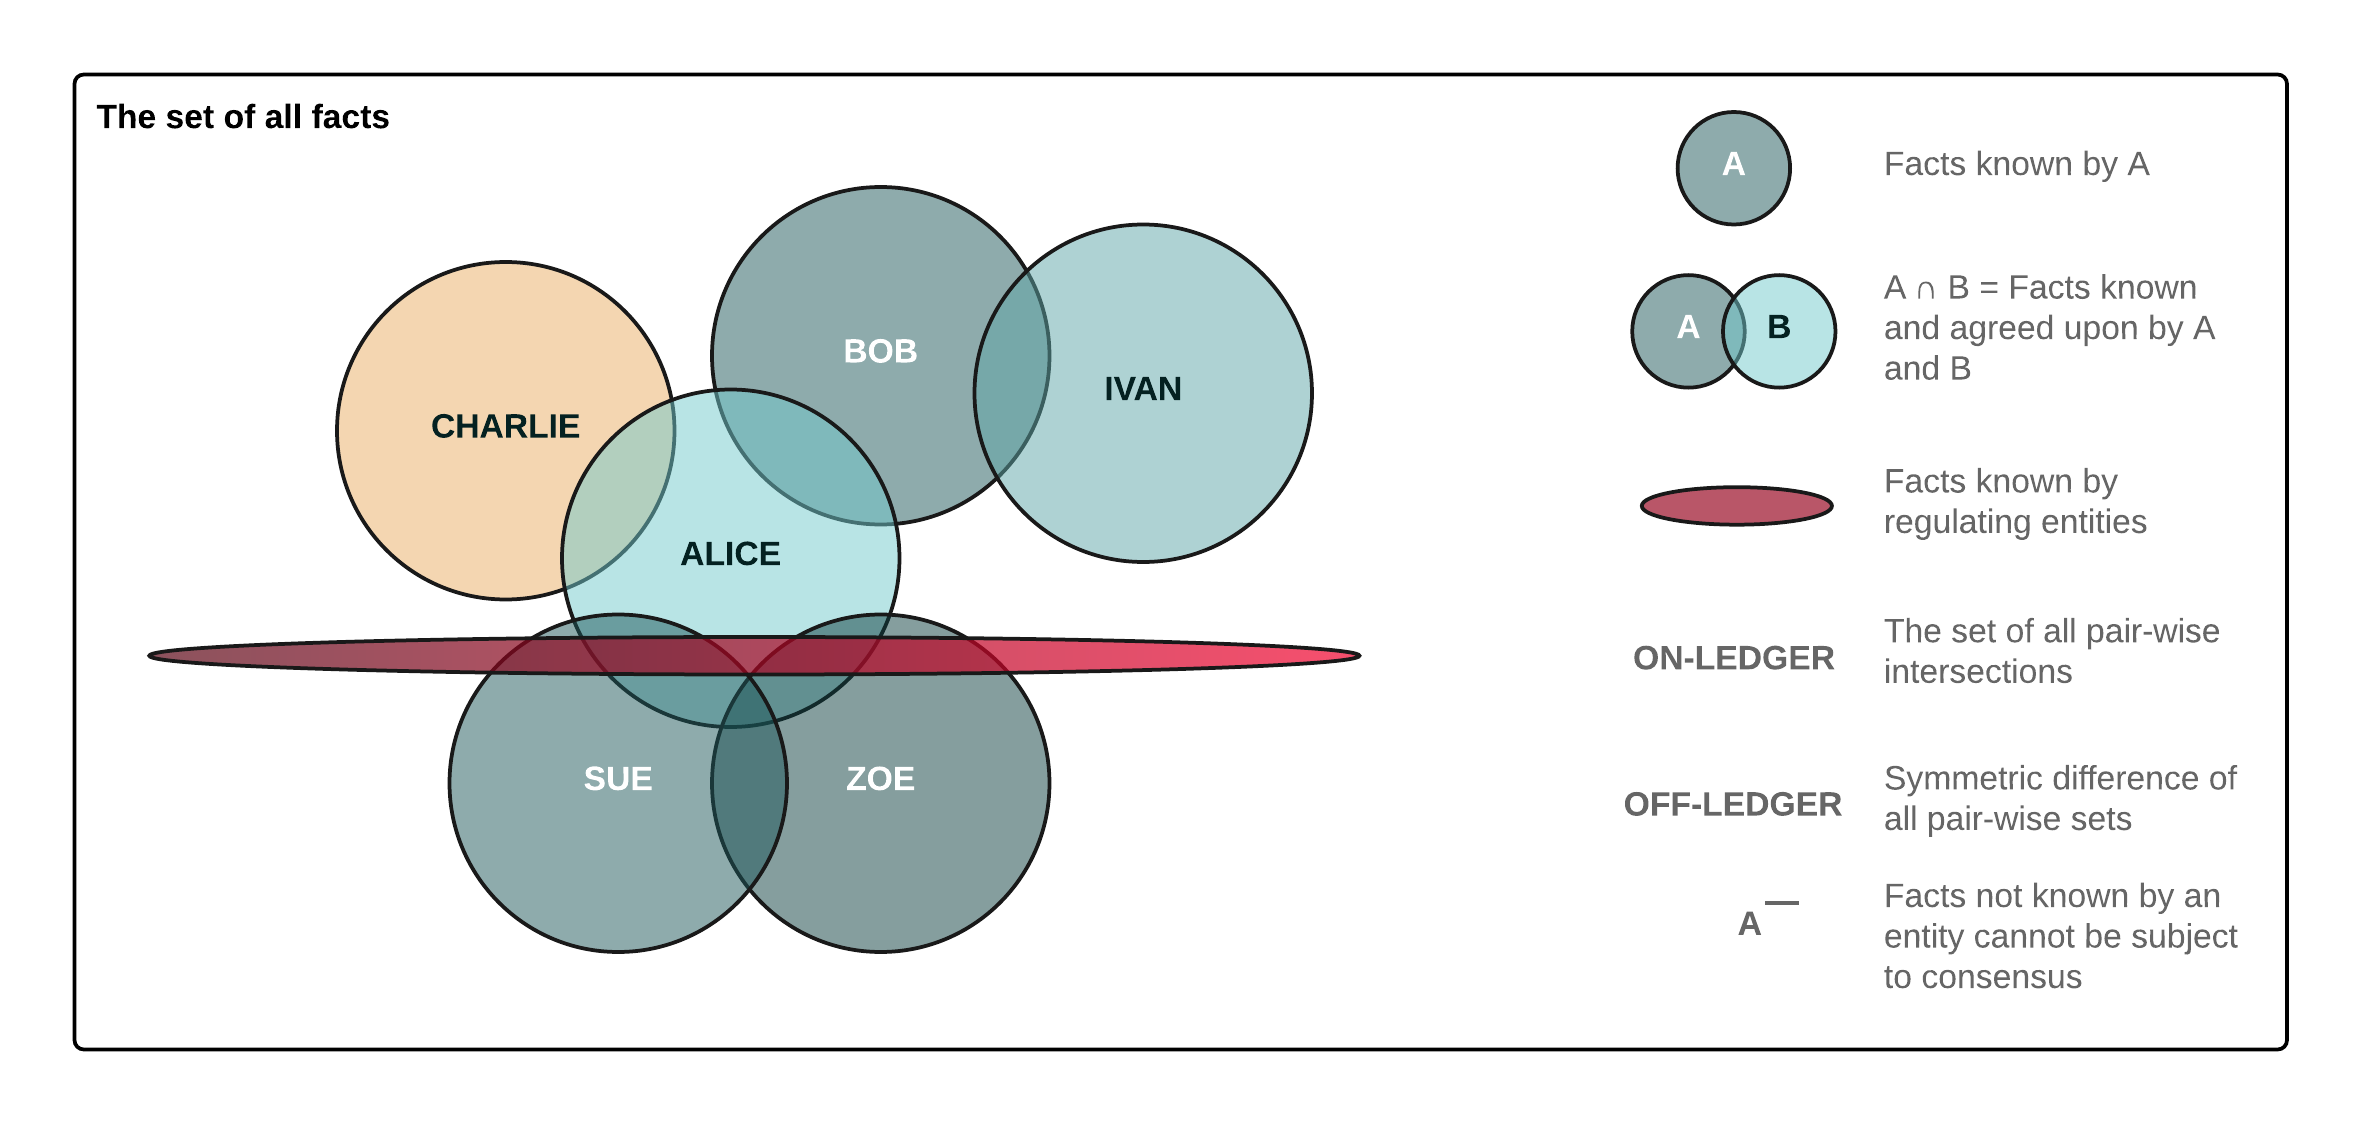
\includegraphics[scale = .5, center]{Consensus}
    \caption{Consensus over transaction validity is performed only by parties to the transaction in question. Therefore, data is only shared with those parties which are required to see it. Other platforms generally reach consensus at the ledger level. Thus, any given actor in a Corda system sees only a subset of the overall data managed by the system as a whole. We allow arbitrary combinations of actors to participate in the consensus process for any given piece of data.}
\end{figure}

Corda has ``pluggable" uniqueness services. This is to improve privacy, scalability, geographic availability, legal-system compatibility\cite{EUC} and algorithmic agility. A single service may be composed of many mutually untrusting nodes coordinating via a byzantine fault tolerant algorithm, or could be very simple, like a single machine.

It is important to note that these uniqueness services are required only to attest as to whether the states consumed by a given transaction have previously been consumed; they are not required to attest as to the validity of the transaction itself, which is a matter for the parties to the transaction. This means that the uniqueness services are not required to (and, in the general case, will not) see the full contents of any transactions, significantly improving privacy and scalability of the system compared with alternative distributed ledger and blockchain designs.  This design decision represents an important choice as to the acceptable tradeoffs in shared ledger architectures and is explored more fully in the technical whitepaper.

\subsection{Business Logic}
Corda enforces business logic through smart contract code. A smart contract in Corda is a pure function whose responsibility is either to accept or reject a proposed transaction and which can be composed from simpler, reusable functions. Each state object specifies the function that must be executed by any transaction which seeks to consume or create that type of state. As such, for any given proposed transaction, one of these functions is executed for each type of state in that transaction, and all must agree that the proposed transaction is permissible given the rules associated with each state. Thus a transaction is valid only if the contract code associated with all contained states agree. It is the responsibility of a transaction proposer to construct a transaction which complies with the constraints associated with each included state object. Contracts thus define the consensus-critical part of the business logic of the ledger, and they are mobile: nodes will download and run contracts inside a sandbox without any review in some deployments, although we envisage the use of signed code for deployments on the global Corda network. This model, whereby one party proposes a transaction and others verify it, is modelled on Bitcoin (albeit heavily extended and generalised) and is the key to Corda's privacy and scalability characteristics.

The virtual machine we have selected for contract execution and validation is the Java Virtual Machine\cite{JVM}, as it has a wealth of existing libraries and a large skill base, and reusing an industry standard makes it easier for banks to reuse their existing code inside contracts. However, we augment it with a custom sandbox that is radically more restrictive than the ordinary JVM sandbox, and it enforces not only security requirements but also deterministic execution. Like Ethereum\cite{Ethereum}, the choice of standardising a bytecode set rather than a language enables users to innovate in contract language design, or reuse well known languages, according to taste. It also makes it easy to directly use contract code from internal applications, once that contract has been reviewed, which should simplify application development considerably.

\subsection{Identity}
Corda enables a broad range of identities to participate in transactions, from institutions to individuals. An identity in Corda is represented by a certificate, signed by a suitable authority, representing a named real-world actor. Participants are expected to protect the private keys associated with their Corda identities, and transactions signed by a participant's key are intended to be legally binding on that participant.

Corda implements its core identity framework through the use of X.509 certificates. This enables Corda to associate a unique ``human readable" entity name (i.e. a legal name) with a public key and network address (IP address). Corda strictly requires uniqueness in this mapping. An entity ``distinguished name" (for example that of a company or legal person) can be associated with at most one public key. This is for non-repudiation purposes so a transaction signature can be legally and unambiguously associated with a legal entity, and to eliminate sources of ambiguity in user interfaces and elsewhere. Upon this foundation can be layered value added services from multiple providers.

The underlying Corda software assumes an identity infrastructure between the participants in the network but makes no assumption as to its sophistication or mode of operation; the global Corda network introduces a specific model, optimised for broad access whilst rigorously ensuring the uniqueness of issued certificates needed to enable formation of real-world legal contracts.

\subsection{Summary of the Corda Model}
The core concepts in our model are:
\begin{itemize}

\item \textit{State objects}, representing an agreement between two or more parties, governed by machine-readable \textit{Contract Code}. This code references, and is intended to implement, portions of human-readable \textit{Legal Prose}. \item \textit{Transactions}, which transition state objects through a lifecycle.
\item A \textit{Flow Framework}, which enables parties to coordinate actions without a central controller.
\end{itemize}

Determinism is achieved, and the amount of shared state required minimized by selectively and decisively restricting the universe of allowable programming techniques.

The combination of state objects (data), Contract Code (constraints on the evolution of that data), the Flow Framework (business logic choreography), any necessary APIs, wallet plugins, and UI components can be thought of a Shared Ledger application, or Corda Distributed Application (\textit{``CorDapp"}). This is the core set of components a contract developer on the platform should expect to build.

\begin{figure}[H]
    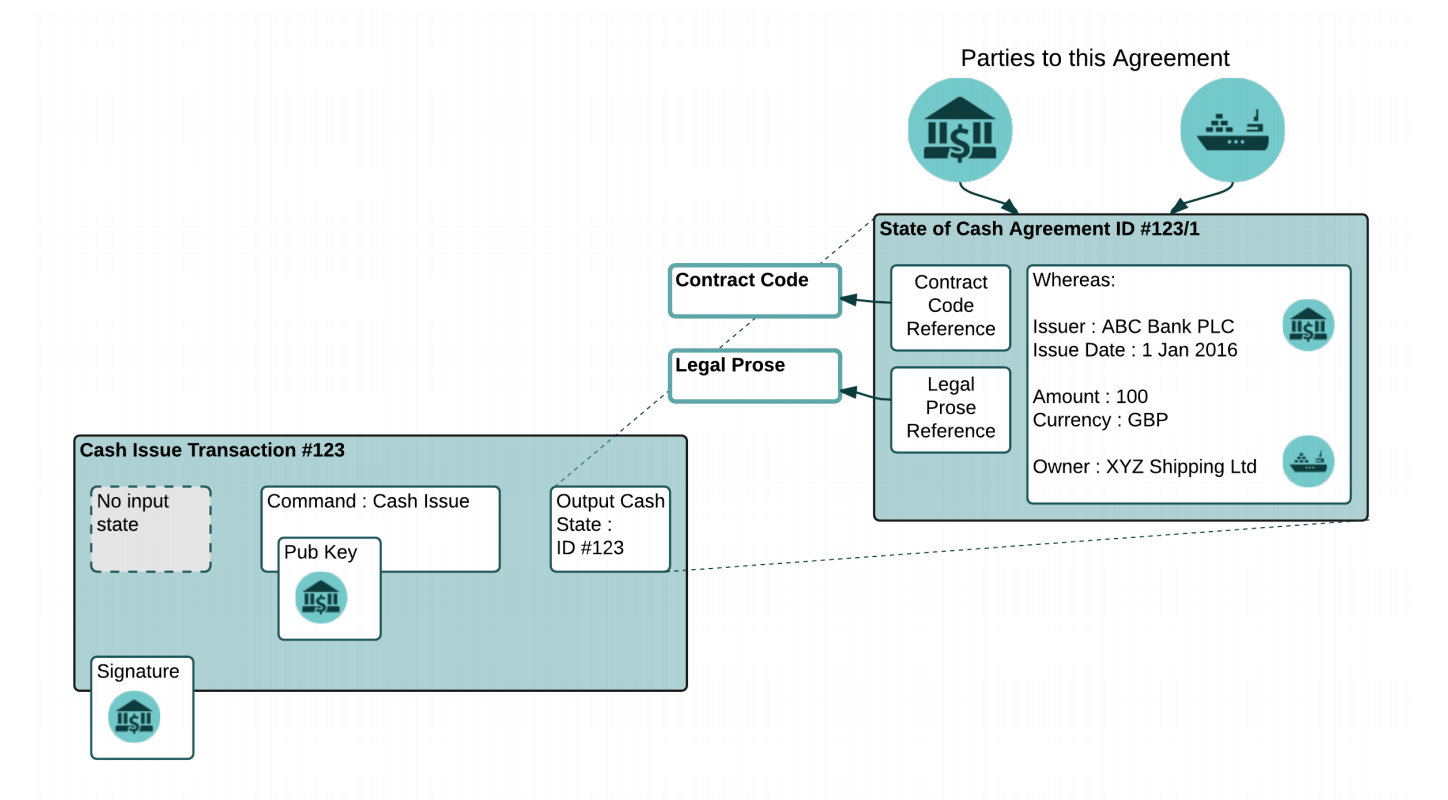
\includegraphics[scale = .4, center]{cash}
    \caption{In the diagram above, we see one of the simplest Corda transactions: a cash issuance transaction.  We see the creation of a new Cash state, issued by a commercial bank to a fictional shipping company. The issuing transaction is signed by the issuing bank.  From this simple model, significantly more complicated transactions, such as payments, delivery-versus-payment contracts and future-dated obligations can be constructed.}
\end{figure}

\section{The Global Corda Network}
The global Corda network consists of the set of nodes in the world that are configured with common settings such that they can locate each other, with assured identity, to transact directly. The network provides the standards needed to allow Corda nodes to transact flawlessly regardless of who operates them, which applications they run, in which trading groupings they participate, and regardless of the original reason for their deployment. The network enables the formation of an open ecosystem where services can be offered both to specific groups of nodes (``business networks", as distinct from the global Corda network itself), or to all nodes. The network provides an open environment for the deployment of Corda nodes with transaction legality, finality and privacy. The network is underpinned by a governance model intended to ensure it operates in the interest of its participants.

\subsection{Business Networks} \label{businessnetworks}
We anticipate that most deployments of Corda will consist of parties coming together to automate one or more common business processes, and these deployments will be underpinned by specific business models and membership criteria. We refer to such a collection of parties as a business network: a group of Corda network participants who collaborate for a specific business purpose whilst nevertheless being able to participate in other business networks or transact directly with other nodes at the same time and with the same infrastructure. The Corda network provides the capability to form business networks while allowing participants to remain unconstrained in their ability to move assets or form agreements freely.

Business networks define their own membership criteria, privacy requirements, governance, business logic and asset types. Participants can be members of many business networks as well as transacting directly with arbitrary peers.

The global Corda network is intended to enable a large number of overlapping, competing and collaborating Business networks to form, unified by just enough commonality to facilitate interoperability of nodes, and compatibility of assets and other contracts managed by those nodes.

Business networks will play a key role in the health of the Corda network ecosystem providing the mechanism through which CorDapps are rooted in the regulatory and legal aspects of various legal jurisdictions.

\begin{figure}[H]
    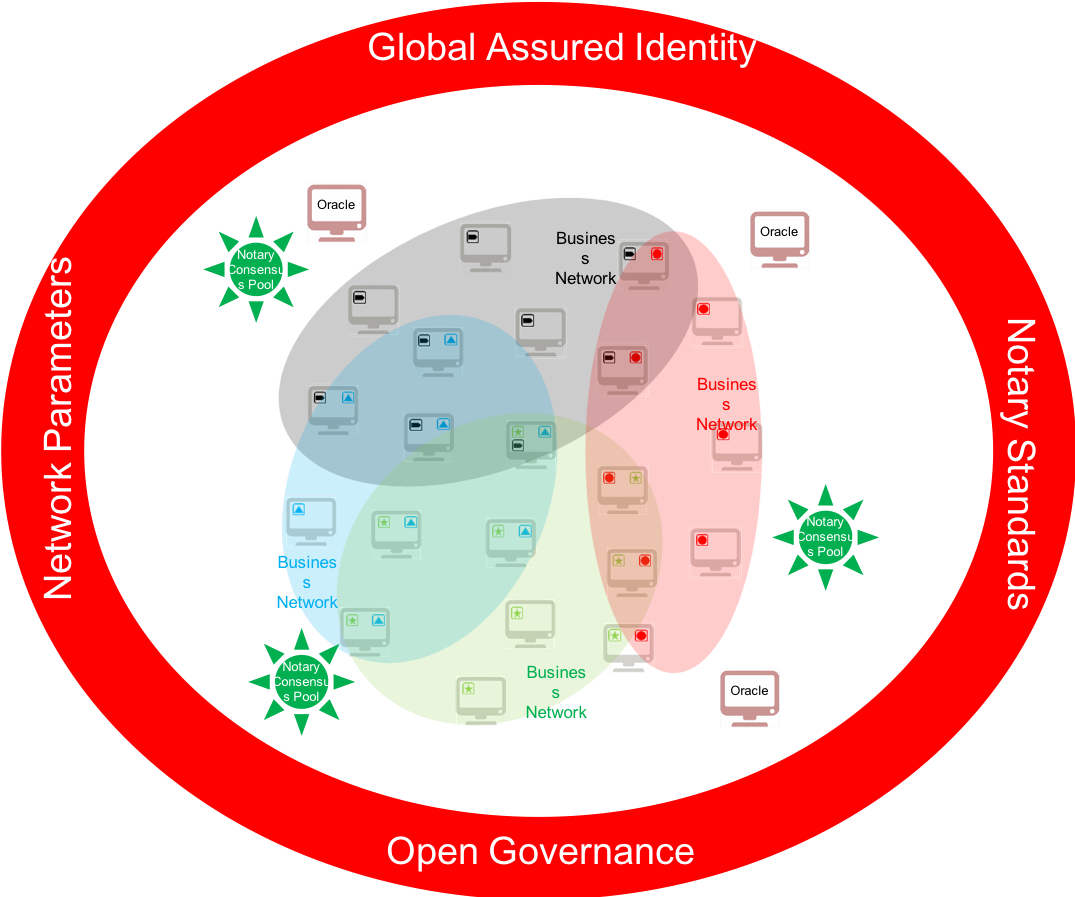
\includegraphics[scale = .5, center]{corda-connect}
    \caption{The global Corda network: seamless interoperability, and frictionless commerce, through shared standards and open governance.}
\end{figure}

\subsection{Principal Components}

The global Corda network:
\begin{itemize}
    \item specifies \textit{network parameters} that define the consensus-critical settings nodes must agree on to ensure global compatibility and stability
    \item provides \textit{an identity framework} so firms can enter into real-world contracts with confidence
    \item recommends \textit{consensus pools} that provide consistent, transparent and resilient uniqueness consensus services
    \item enables \textit{oracles} that provide information services across the network
    \item facilitates \textit{fiat currencies} and \textit{native digital tokens} in a standard representation for seamless transfer of value
    \item relies on \textit{open governance} that represents the stakeholders of the Corda ecosystem
\end{itemize}

\subsubsection{Governance}

Whilst the overwhelming majority of power lies with Corda users themselves, or the governors of their chosen business networks, some residual control unavoidably lies in the specification of the standards and operation of associated technical services upon which all participants rely. This means the success of the Corda network depends on the extent to which it is operated in the interests of its broad base of stakeholders, and is responsive to their needs.

For example, in Bitcoin, the size of the maximum permitted block is ultimately arbitrary within some boundaries. Yet it is an arbitrary figure upon which all participants in \textit{the} Bitcoin network must agree. In the absence of a well thought through and administered governance process to decide on settings such as this, operated by and for the participants in the network, gridlock or conflict can be the result. To avoid a similar outcome, the purpose of the Corda network's governance process is to ensure it is always clear how such disputes can be mediated, by whom and in whose interests.

However, in the end-state of this vision, a huge number of nodes and business networks will be transacting significant volumes of business and value across the global Corda network. So it is not sufficient merely to \textit{claim} that the Corda network will be operated for the benefit of its users. It must be the case that it \textit{will} be so operated. Channeling Google's ``don't be evil" mantra, our vision for the Corda network is that it be operated so that it \textit{can't be evil}.

To that end, an open governance model will be established in a series of stages and effected through a ``Corda network governing body", whose composition is intended to be representative of the users of the Corda network. The committee's responsibilities will include: to take over the definition, management and updating of network parameters; to agree rules for the issuance of identity certificates; and to set common standards for notary consensus pools.

\subsubsection{Network Parameters}

Corda users need to agree on certain technical parameters that must be the same for all nodes in order to communicate successfully. Examples include the maximum-allowable message size, how quickly members agree to upgrade their nodes when a new feature is introduced, and how to use privacy features like Intel SGX. Although these sound like unimportant technical points, they are configuration parameters of the Corda software precisely \textit{because} they are things upon which reasonable people could disagree, as happened with the Bitcoin block size debate. As such, the parameter-setting process could rapidly become politicised. It is, therefore, a priority to move responsibility for setting, maintaining and updating these parameters to the Corda network governing body once established.

\subsubsection{Identity}

Corda manages real contracts between real people and firms. So we need a way for users to know they really are transacting with who they think they are. This requires there to be a unique mapping from real-world identity to network identity (public key). As such, it is an unavoidable consequence that an important network parameter is which identity authority or authorities to rely on.

However, it is our vision that access to the Corda network be available to as broad a range of participants as possible; restrictions driven by business model, regulation or geography can and should be implemented at the level of individual business networks, not at the level of the overall platform. Indeed, it is important to emphasise that operators of business networks are able, and indeed are expected, to independently verify participants' identities before admitting them to their business networks. It is this extra layer of checking that allows the Corda network-level identity framework to be as light as possible whilst ensuring uniqueness of identity certificates.

To this end, the Corda network will launch with a simple identity service that will subsequently be upgraded to enable a broader range of approaches. One such approach is likely to be one where participants ``bring their own identity" in the form of signed attestations from a set of trusted identity issuers/attestors. We envisage a model whereby the automatic issuance of a Corda network certificate can be triggered for any party with the requisite attestations, subject only to the constraint that any resulting identity certificate issued on the global Corda network is unique, both for the distinguished name and the public keys or any other unique identifier that may be used in the future.

One of the responsibilities of the Corda network governing body will be to oversee this process, including setting standards for attestors. We expect this deliberately minimal identity framework to catalyse the formation of a rich ecosystem of identity value added services through third party specialist providers which can layer on top of this foundation to meet the varying needs of different applications.

\subsubsection{Consensus}

Corda, like all blockchain platforms, works on the principle of \textit{consensus}. Parties know a transaction has been confirmed when the appointed consensus service has processed it. Uniquely, Corda is architected to support volumes in excess of billions of daily transactions across a single network. To achieve this, Corda allows for a range of consensus services (notary pools) optimised for different purposes on the same network, including on the global Corda network described in this chapter.

Participants can verify the integrity of these choices through a variety of mechanisms: some notary pools will provide transparency (in a way analogous to public blockchains today). Others may remotely attest that they are running a particular algorithm in a secure enclave. To aid network participants in configuring their nodes and to maximise interoperability, a responsibility of the Corda network governing body is to establish and maintain a list of notary pools which are considered to be operated to sufficient standards of integrity. Participants are encouraged to configure their nodes to accept historical transactions that have been notarised by pools on this shared list to maximise compatibility of transactions across the network. Participants can, of course, choose any notary pool to notarise their own transactions; this shared list is to enable historic transactions to be easily combined with new transactions to enable free movement of data and assets around the network; the fundamental vision and unique characteristic of Corda.

\subsubsection {The Corda Network Economic Model}

The success of Corda and the global Corda network depends, in part, on there being a vibrant ecosystem of participants on the network: users; designers, governors and operators of business networks; application developers; providers of notary nodes; oracle services and infrastructure providers, many of whom will need to pay and be paid.

The global Corda network will support a digital representation of fiat money, the first broad-access blockchain network to do so. However, access to this facility will necessarily be subject to the thicket of regulation that attaches to the global payments system.

Therefore, the Corda network may also offer support for an asset which is native to the platform and which can be far more broadly held, subject to regulatory approval.

The Corda network can encourage the emergence of application-specific native assets or tokens, utilising a common standard for representation, storage and exchange of such tokens.

\section{Comparisons with Other Platforms}
Corda's design is  inspired by previous work, including that introduced in the writings of Todd Boyle and Ian Grigg on triple entry accounting\cite{Triple}, and aspects of existing distributed ledger platforms such as Bitcoin\cite{Bitcoin} and Ethereum. We can compare our vision with two alternative models: the public blockchains and the enterprise blockchains.

\begin{figure}[H]
    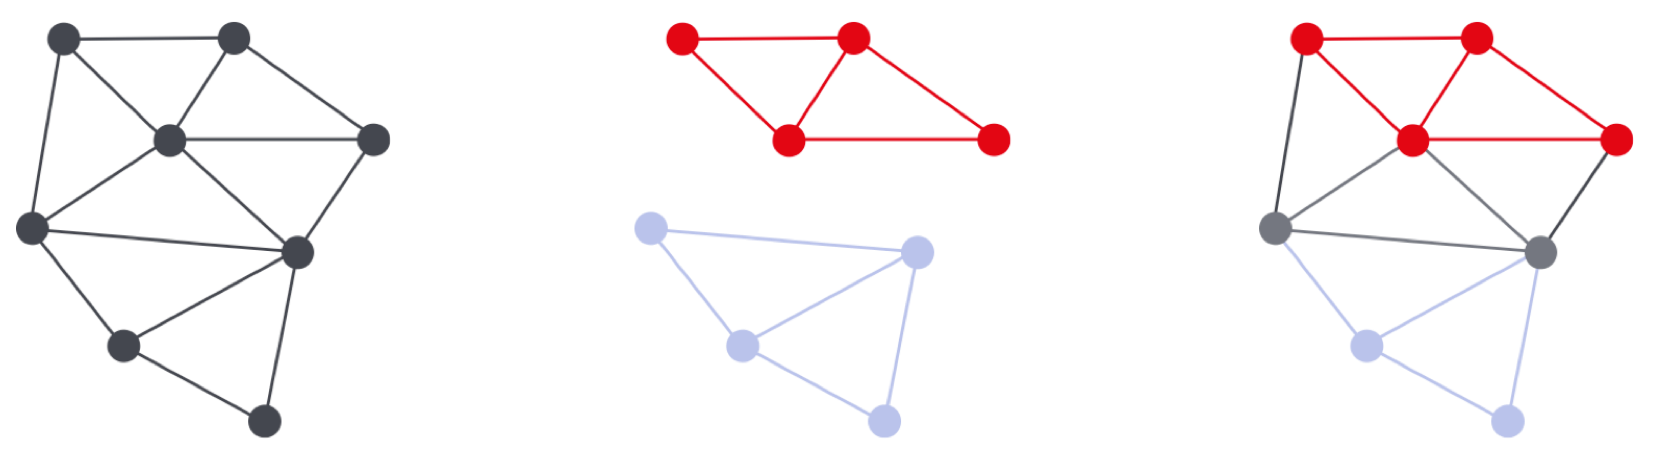
\includegraphics[scale = .5, center]{platform-comparisons}
    \caption{Corda delivers the promise of interoperable applications in an enterprise context (right) without the disadvantages of the fully public Ethereum network (left) or the non-interoperable, expensive standalone networks being built by first-generation enterprise blockchains (middle).}
\end{figure}

\subsection{Comparisons to Public Blockchains: Bitcoin and Ethereum}

The first diagram above is the model enabled by Bitcoin and delivered by Ethereum: a single global network upon which large numbers of users and applications can transact and interoperate. It is a compelling vision and has rightly captured the imagination of many enthusiasts.  Unfortunately, it suffers from severe drawbacks when applied to the enterprise domain: all data is shared with all parties, with obvious privacy and scalability implications, and no realistic prospect in sight of a truly workable solution. For this reason and others it is proving exceedingly difficult to adapt or adopt the public Ethereum architecture for enterprise use-cases. Specific comparisons to Bitcoin and Ethereum now follow:

\subsubsection{Comparisons to Bitcoin}
Corda has some significant similarities to Bitcoin:
\begin{itemize}
\item{Immutable states that are consumed and created by transactions is the same.}
\item{Transactions have multiple inputs and outputs. Bitcoin sometimes refers to the ledger as the unspent transaction output set (UTXO set) as a result. However, the Corda model is a significant generalisation of this concept, to support arbitrarily complex data models.}
\item{A contract is pure function; contracts do not have storage or the ability to interact with anything. Given the same transaction, a contract's ``verify" function always yields exactly the same result.}
\end{itemize}

However, a Bitcoin transaction has a single, rigid data format and can hold very little data apart from quantities of bitcoin and associated spending rules (script). Some people have been known to try and work around this limitation by embedding data in semi-standardized places in the contract code so the data can be extracted through pattern matching but this is a poor approach.

By contrast, our states can include arbitrary typed data. In addition, our transactions invoke not only input contracts but also the contracts of the outputs. A Bitcoin transaction's acceptance is controlled only by the contract code in the consumed input states. We use the term ``contract" to refer to a bundle of business logic that may handle various different tasks, beyond transaction verification. For instance, currently our contracts also include code for creating valid transactions (this is often called ``wallet code" in Bitcoin).


A Bitcoin script can only be given a fixed set of byte arrays as the input. This means there is no way for a contract to examine the structure of the entire transaction, which severely limits what contracts can do. Our contracts are Turing-complete and can be written in any ordinary programming language that targets the JVM.

Corda allows arbitrarily-precise time-bounds to be specified in transactions (which must be attested to by a trusted timestamper) rather than relying on the time at which a block happens to be mined.  This is important given that many contract types we envisage supporting require precision in timing and because our primary consensus implementations use block-free conflict resolution algorithms. It should be noted that Corda does not utilise Proof of Work or have a concept of ``mining".

\subsubsection{Comparisons to Ethereum}
Like Ethereum, CorDapp code runs inside a relatively powerful virtual machine and can contain complex logic. Non-assembly based programming languages can be used for contract programming.  They are both intended for the modelling of many different kinds of financial contracts.

However, the term ``contract" in Ethereum refers to an instantiation of a program that is replicated and maintained by every participating node. This instantiation is very much like an object in an Object Oriented program: it can receive and send messages, update local storage and so on. In contrast, our implementation of the smart contract in code refers to a set of functions, only one of which is a part of keeping the system synchronised (the \textit{verify} function). That function is pure and stateless (i.e., it may not interact with any other part of the system whilst executing).	As contracts do not have any kind of mutable storage, there is no notion of a ``message". This model means it is possible to analyse a Corda transaction statically and not only determine whether it can be processed in parallel with other transactions but know what data must be available on the processing node, enabling both higher throughput and finer-grained data privacy.

\subsection{Comparisons to Enterprise Blockchains: Enterprise Ethereum and Hyperledger Fabric}

The second model, drawn in the centre of the diagram above is the inevitable result of efforts that have tried to apply the Ethereum architecture to enterprise use-cases. With Enterprise Ethereum platforms such as Quorum as well as clones of Ethereum such as Fabric, we see a wholesale retreat from the vision: each business solution is deployed as an independent, standalone network that is incompatible with all the others, completely undermining a key foundation of the value proposition.  Assets earned on one of these networks will not be easily usable on another. Each silo will require its own identity, consensus and governance processes.  The firms who deploy nodes to connect to these networks will be lumbered with expensively duplicated and incompatible infrastructure in their data-centres. And the industry will then have to spend millions of dollars inventing ways to make these isolated networks interoperate with each other. This is the complete opposite of what the enterprise blockchain revolution is intended to deliver.

\section{Conclusion}

In contrast to most existing distributed ledger and blockchain platforms today, Corda was built with the explicit purpose of recording and enforcing business agreements between trading partners. As such, it takes a unique approach to data distribution and transaction semantics while emphasising the features of distributed ledgers which are attractive to firms, namely reliable execution of contracts in an automatable and enforceable fashion.

The Corda vision, enabled by the global Corda network, enables multiple applications and services to run across a common layer of identity, consensus, business logic, data definitions, and governance. Firms can deploy one Corda node infrastructure which can then transact with multiple different groups of trading partners, for different purposes, all at the same time and whilst providing strong privacy. Multiple different competing notary consensus pools, comprised of a range of providers, will be available; data and other oracle services can be deployed once and used by multiple applications; and the entire ecosystem will be governed by and for its users through a transparent and open process.  Multiple different applications, designed for completely different purposes, can be deployed today to solve specific problems and yet, in the future, contracts and other information managed by these applications could be combined in new ways for purposes unimaginable today.

\bibliographystyle{unsrt}

\bibliography{Ref}

\end{document}
